\chapter{Descrição da Prática e Análise Teórica}

Para viabilizar a análise do conversor \textit{Buck} utilizando o arcabouço matemático da Teoria de Circuitos Lineares, é imperativo que todos os componentes do circuito operem de maneira linear. Como o circuito real possui componentes de chaveamento semicondutores não-lineares, a abordagem adotada divide a operação em janelas de tempo discretas, tratando cada estado da chave como um subcircuito linear independente.

\section{Modelagem Matemática do Diodo}

O diodo é um dispositivo inerentemente não-linear cuja condução depende da polaridade da tensão aplicada em seus terminais. Para evitar a complexidade das equações exponenciais do diodo real (equação de Shockley) na Transformada de Laplace, adotou-se um modelo linear por partes (\textit{piecewise linear}).

As Figuras \ref{fig:diodo_simbolo} e \ref{fig:diodo_curva} ilustram o símbolo do dispositivo e a sua curva característica de aproximação adotada para esta análise. 

\begin{figure}[H]
	\centering
	\begin{minipage}{0.45\textwidth}
		\centering
		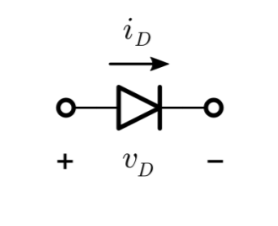
\includegraphics[width=0.7\textwidth]{FIGURAS/representacao_gráfica_diodo.png}
		\caption{Representação gráfica do diodo e suas polaridades de referência.}
		\label{fig:diodo_simbolo}
	\end{minipage}\hfill
	\begin{minipage}{0.45\textwidth}
		\centering
		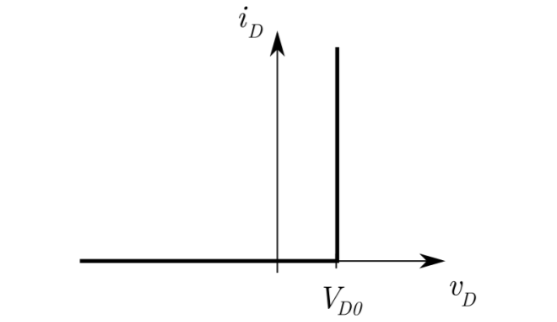
\includegraphics[width=0.9\textwidth]{FIGURAS/modelo_curva_tensão_corrente.png} 
		\caption{Curva tensão-corrente do modelo linear por partes.}
		\label{fig:diodo_curva}
	\end{minipage}
\end{figure}

Matematicamente, este modelo determina que, a cada instante de tempo, o diodo opera estritamente em uma de duas regiões:
\begin{itemize}
	\item \textbf{Polarização Reversa ($v_D < V_{D0}$):} O diodo atua como uma chave aberta. A corrente é nula ($i_D = 0$) e a resistência equivalente tende ao infinito.
	\item \textbf{Polarização Direta ($i_D > 0$):} O diodo conduz e atua como uma fonte de tensão ideal e constante, de valor $V_{D0}$, em oposição à corrente.
\end{itemize}

\section{O Conversor \textit{Buck} Simplificado}

O circuito sob estudo consiste em uma versão simplificada do conversor \textit{Buck}, desprovida do capacitor de filtro na saída, conforme ilustrado na Figura \ref{fig:modelo_buck}. O arranjo é composto por uma fonte de tensão contínua ($V_{CC}$), uma chave de estado sólido, um diodo de roda livre, um indutor ($L$) e uma resistência de carga ($R$).

\begin{figure}[H]
	\centering
	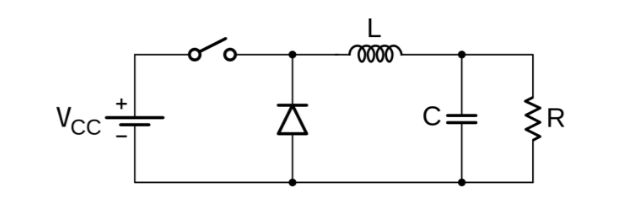
\includegraphics[width=0.6\textwidth]{FIGURAS/modelo_buck.png}
	\caption{Esquemático do conversor \textit{Buck} simplificado adotado para a análise teórica.}
	\label{fig:modelo_buck}
\end{figure}

A chave do circuito é submetida a um sinal de controle tipo onda quadrada de período $T$. Ela permanece fechada durante um tempo $kT$ e aberta pelo restante do período $(1-k)T$, onde $k$ é o ciclo de trabalho (\textit{duty cycle}). 

Aplicando a modelagem do diodo, o circuito transmuta-se entre duas topologias lineares distintas, que devem ser analisadas individualmente no domínio de Laplace ($s$). Para modelar a transição entre os estados, a corrente final do indutor em uma etapa torna-se a corrente inicial ($i_L(0^-)$) da etapa subsequente.

\section{Análise no Domínio de Laplace}

\subsection{Estado 1: Operação com a Chave Fechada ($0 \le t < kT$)}

Quando a chave é fechada, a tensão $V_{CC}$ impõe um potencial positivo no cátodo do diodo, forçando-o a operar na região de \textbf{polarização reversa}. Logo, o diodo comporta-se como um circuito aberto. O subcircuito resultante é um laço série contendo a fonte $V_{CC}$, o indutor $L$ e o resistor $R$.

Assumindo que, no instante em que a chave fecha, a tensão inicial sobre o resistor seja $V_0$, a corrente inicial no indutor é dada pela Lei de Ohm: $i_L(0^-) = V_0 / R$.

Aplicando a Lei de Kirchhoff das Tensões (LKT) no domínio da frequência $s$ e incorporando a condição inicial do indutor como uma fonte de tensão em série de valor $L \cdot i_L(0^-)$, obtemos:

\begin{equation}
	\frac{V_{CC}}{s} = L \left( sI(s) - \frac{V_0}{R} \right) + R \cdot I(s)
\end{equation}

Isolando a corrente $I(s)$ algebricamente:

\begin{equation}
	\frac{V_{CC}}{s} + \frac{L \cdot V_0}{R} = I(s) (sL + R) \implies I(s) = \frac{\frac{V_{CC}}{s} + \frac{L \cdot V_0}{R}}{sL + R}
\end{equation}

A variável de interesse é a tensão sobre a carga $V_{Rf}(s)$ (onde o sufixo $f$ denota chave \textit{fechada}). Sendo $V_{Rf}(s) = R \cdot I(s)$, e processando a expansão dessa expressão racional com a rotina computacional simbólica do Maxima \cite{maxima}, encontra-se:

\begin{equation}
	V_{Rf}(s) = \frac{V_{CC} \frac{R}{L}}{s \left(s + \frac{R}{L}\right)} + \frac{V_0}{s + \frac{R}{L}}
\end{equation}

Aplicando a Transformada Inversa de Laplace (\texttt{ilt()}) para retornar ao domínio do tempo, a tensão durante o período em que a chave está fechada resulta na expressão:

\begin{equation}
	v_{Rf}(t) = V_{CC} \left(1 - e^{-\frac{R}{L}t}\right) + V_0 e^{-\frac{R}{L}t}
\end{equation}

\subsection{Estado 2: Operação com a Chave Aberta ($kT \le t < T$)}

Ao abrir a chave em $t = kT$, a fonte $V_{CC}$ é desconectada. Contudo, a propriedade inercial do indutor exige a continuidade da corrente. Essa corrente força o diodo a conduzir, colocando-o no modo de \textbf{polarização direta}. O diodo passa a atuar como uma fonte ideal $V_{D0}$, fechando a malha de circulação ("roda livre") para a energia armazenada no indutor. 

Redefinindo o eixo de tempo de forma que a abertura da chave corresponda a $t = 0$, e sabendo que a tensão na carga nesse exato momento é $V_1$, a nova condição inicial de corrente no indutor será $i_L(0^-) = V_1 / R$.

Aplicando a LKT em Laplace na malha de roda livre:

\begin{equation}
	-\frac{V_{D0}}{s} = L \left( sI(s) - \frac{V_1}{R} \right) + R \cdot I(s)
\end{equation}

Isolando a corrente $I(s)$:

\begin{equation}
	-\frac{V_{D0}}{s} + \frac{L \cdot V_1}{R} = I(s) (sL + R) \implies I(s) = \frac{-\frac{V_{D0}}{s} + \frac{L \cdot V_1}{R}}{sL + R}
\end{equation}

Multiplicando pela resistência de carga ($R$) para encontrar a tensão de saída com a chave aberta ($V_{Ra}(s)$) e aplicando as manipulações no Maxima \cite{maxima}, obtém-se:

\begin{equation}
	V_{Ra}(s) = \frac{-V_{D0} \frac{R}{L}}{s \left(s + \frac{R}{L}\right)} + \frac{V_1}{s + \frac{R}{L}}
\end{equation}

A Transformada Inversa de Laplace desta função racional revela a resposta transitória temporal da descarga da bobina durante o estado aberto:

\begin{equation}
	v_{Ra}(t) = -V_{D0} \left(1 - e^{-\frac{R}{L}t}\right) + V_1 e^{-\frac{R}{L}t}
\end{equation}

\section{Dinâmica Periódica e Regime Permanente}

Devido ao chaveamento contínuo, as tensões $v_{Rf}(t)$ e $v_{Ra}(t)$ alternam-se, moldando a tensão final na carga. A continuidade da corrente no indutor impõe que a tensão de saída não sofra descontinuidades abruptas nas transições. O formato de onda global originado por essas parcelas exponenciais em carga e descarga pode ser visualizado na Figura \ref{fig:onda_periodo}.

\begin{figure}[H]
	\centering
	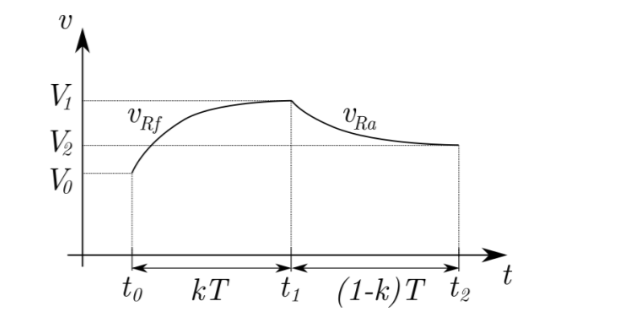
\includegraphics[width=0.7\textwidth]{FIGURAS/tensão_saída_período_onda_quadrada_controle_chave.png}
	\caption{Evolução temporal da tensão no resistor de carga $v_R(t)$ ao longo de um período de chaveamento.}
	\label{fig:onda_periodo}
\end{figure}

A partir destas equações temporais e da continuidade entre os estados limites ($V_0 \to V_1$ e $V_1 \to V_2$), é possível estender o formalismo matemático para estabelecer as métricas do regime permanente do conversor ($V_0$ constante e $\Delta V$), bem como aproximar o \textit{ripple} por meio de expansões de Taylor para ciclos de chaveamento suficientemente rápidos ($T \to 0$).



\section{Avaliação das Tensões de Comutação ($V_1$ e $V_2$)}

Para compreender o comportamento do conversor, avaliam-se as tensões nos momentos exatos de comutação da chave. Denota-se $V_1$ como a tensão na carga no exato momento em que a chave abre (final do período de condução, $t = kT$) e $V_2$ como a tensão no momento em que a chave fecha novamente (final do período de roda livre, transcorrido um tempo extra de $(1-k)T$).

Substituindo estes instantes de tempo nas funções temporais $v_{Rf}(t)$ e $v_{Ra}(t)$ obtidas via Transformada Inversa de Laplace, têm-se as tensões de contorno:

\begin{equation}
	V_1 = v_{Rf}(kT) = V_{CC} \left(1 - e^{-\frac{R}{L}kT}\right) + V_0 e^{-\frac{R}{L}kT}
	\label{eq:v1}
\end{equation}

\begin{equation}
	V_2 = v_{Ra}((1-k)T) = -V_{D0} \left(1 - e^{-\frac{R}{L}(1-k)T}\right) + V_1 e^{-\frac{R}{L}(1-k)T}
	\label{eq:v2}
\end{equation}

\section{Análise em Regime Permanente}

Em regime permanente, as correntes e tensões do circuito entram em um ciclo estacionário, o que significa que o estado final de um período é idêntico ao estado inicial daquele mesmo período. Portanto, a tensão na carga no final do ciclo ($V_2$) deve ser igual à tensão no início do ciclo ($V_0$). Impondo a condição $V_2 = V_0$ na Equação \ref{eq:v2} e substituindo $V_1$ pela Equação \ref{eq:v1}, o sistema algébrico resolvido fornece a tensão de patamar inferior $V_0$:

\begin{equation}
	V_0 = \frac{-V_{D0} \left(1 - e^{-\frac{R}{L}(1-k)T}\right) + V_{CC} \left(e^{-\frac{R}{L}(1-k)T} - e^{-\frac{R}{L}T}\right)}{1 - e^{-\frac{R}{L}T}}
\end{equation}

A ondulação de tensão no resistor, comumente chamada de \textit{ripple} ($\Delta V$), é a diferença entre o pico máximo ($V_1$) e o vale ($V_0$). Manipulando a Equação \ref{eq:v1}:

\begin{equation}
	\Delta V = V_1 - V_0 = (V_{CC} - V_0) \left( 1 - e^{-\frac{R}{L}kT} \right)
\end{equation}

\subsection{Aproximação Linear para Alta Frequência ($T \to 0$)}

Como o objetivo de um conversor \textit{Buck} é fornecer uma tensão de saída com a menor oscilação possível, opera-se com frequências de chaveamento muito altas (ou seja, período $T$ tendendo a zero). Para analisar matematicamente este limite, aplica-se a expansão em Série de Taylor em torno de $T=0$, onde a exponencial aproxima-se de uma função linear ($e^{-x} \approx 1 - x$).

Aplicando a função \texttt{taylor()} nestas condições, as expressões complexas simplificam-se notavelmente. A tensão média na carga $V_0$ e a ondulação $\Delta V$ tornam-se:

\begin{equation}
	\lim_{T \to 0} V_0 \approx k \cdot V_{CC} - (1-k)V_{D0}
	\label{eq:v0_taylor}
\end{equation}

\begin{equation}
	\lim_{T \to 0} \Delta V \approx (V_{CC} - V_0) \cdot \frac{R}{L} k T
	\label{eq:deltav_taylor}
\end{equation}

A Equação \ref{eq:v0_taylor} evidencia o princípio fundamental do conversor \textit{Buck}: ignorando-se a queda de tensão no diodo ($V_{D0} \approx 0$), a tensão de saída contínua é simplesmente a tensão de entrada multiplicada pelo ciclo de trabalho da chave ($V_0 \approx k \cdot V_{CC}$).

\section{Dimensionamento Numérico do Indutor ($L$)}

A Equação \ref{eq:deltav_taylor} revela que o \textit{ripple} de tensão ($\Delta V$) é inversamente proporcional à indutância $L$ e à frequência de chaveamento ($f = 1/T$). Para mitigar essa oscilação e atender a um requisito de projeto onde $\Delta V$ deve ser estritamente $0,1\%$ da tensão de entrada ($0,001 V_{CC}$), pode-se isolar $L$:

\begin{equation}
	L = \frac{(V_{CC} - V_0) \cdot R \cdot k \cdot T}{\Delta V}
\end{equation}

Assumindo o modelo ideal de diodo ($V_{D0} = 0$) e desejando-se uma tensão de saída equivalente à metade da tensão de entrada ($V_0 = V_{CC}/2$), o ciclo de trabalho necessário é de 50\% ($k = 0,5$). Substituindo $V_0 = 0,5 V_{CC}$, $\Delta V = 0,001 V_{CC}$ e $k = 0,5$, a fórmula geral do indutor de projeto reduz-se a:

\begin{equation}
	L = \frac{(0,5 V_{CC}) \cdot R \cdot 0,5 \cdot T}{0,001 V_{CC}} = 250 \cdot R \cdot T = \frac{250 \cdot R}{f}
\end{equation}

Aplicando esta relação final, calcularam-se os quatro valores nominais de indutância exigidos para as combinações de resistência de carga e frequências de chaveamento solicitadas pelo roteiro, os quais estão compilados na Tabela \ref{tab:calculo_indutor}.

\begin{table}[H]
	\centering
	\caption{Valores teóricos de indutância ($L$) calculados para restringir $\Delta V$ a $0,1\%$ de $V_{CC}$.}
	\label{tab:calculo_indutor}
	\renewcommand{\arraystretch}{1.3}
	\begin{tabular}{ccc}
		\hline
		\textbf{Carga Resistiva ($R$)} & \textbf{Frequência ($f = 10\text{ kHz}$)} & \textbf{Frequência ($f = 50\text{ kHz}$)} \\ \hline
		$5\text{ }\Omega$ & $125\text{ mH}$ ($0,125\text{ H}$) & $25\text{ mH}$ ($0,025\text{ H}$) \\
		$1\text{ }\Omega$ & $25\text{ mH}$ ($0,025\text{ H}$) & $5\text{ mH}$ ($0,005\text{ H}$) \\ \hline
	\end{tabular}
\end{table}

Estes valores dimensionados atuarão como parâmetros de entrada vitais para a etapa subsequente, onde o circuito será simulado computacionalmente.